\documentclass{report}
\usepackage[left=3cm]{geometry}
\usepackage{verbatim}
\usepackage{graphicx}
\usepackage{tabularx}
\setlength{\extrarowheight}{5pt}

\begin{document}
\title{CSE Project}
\author{ALBERT(MINGKUN YANG) ID:900506-T008\\
albertnetymk@gmail.com\\
\maketitle 

\section{Background}
The kernel handles multitasking by Earliest Deadline First(EDF) algorithm. Blocked and unblocked Interprocess Communication(IPC) are supported. One application should be developed to utilize the features.

\section{Project Description}
TCP three-way handshaking is the first step before any TCP based communication, which is fundamental for every student majoring in Computer Science to understand it. This project only tries to simulate the gist of TCP three-way handshaking, which means that message transmitted between the server and the client is much simplified than the real one.

Considering that one server usually maintains several session with different clients simultaneously, we set the number of clients to be greater than 1, so that we utilize the mutltasking function of the kernel and simulate the reality as close as possible.
\section{Specification}
This application stimulates the communication between several clients and one server.

\begin{figure}[p]
  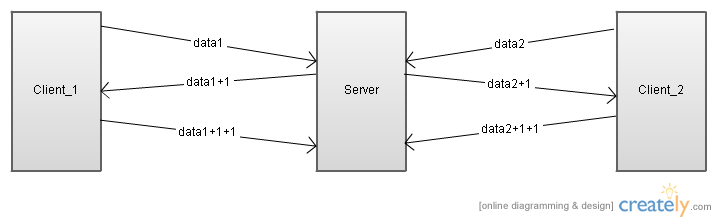
\includegraphics[scale=0.5]{handshaking.png}
  \caption{two clients and one server}
\end{figure}

\begin{table}[p]
  \begin{tabularx}{\textwidth}{| X |}
    \hline
    void task\_server(void) \\
    \begin{itemize}
      \item Sits in one while loop, waiting for clients' request. The number of clients this server can handle is predefined.

      \item Internal while loop to reply client's request one by one, by sending one message to the client. The value contained in this message is based on the value the server received. This value also serves as checksum.

      \item Waits for the client's reply for five cycles, if the server gets the replay, check the return value, otherwise drop this session, which probably can resist the DOS attack to some extent.
      \item If the return value is valid, the server is ready for communication with this client.
    \end{itemize}
    \\

    \hline
    void task\_client(void) \\
    \begin{itemize}
      \item Figure out the index for this invocation according to the deadline

      \item Initializes one session by sending one message to the server.

      \item If it can not get the server's reply after trying for five times, it assumes that the server is down.

      \item When it gets server's reply, compare the value with the value it has sent to check the integrity of the communication.

      \item If the value is valid, generate the new sending value base on the value it received. Now, this client is ready for communication.
    \end{itemize}
    \\
    \hline
  \end{tabularx}
  \caption{Description for tasks in this project}
\end{table}

\section{Discussion}
In close, theoratically, the number of clients can be expanded to any number, easily. However, in that case, the latency will be 
higher. Fortunately, the performance can be tuned by modifying the retry times of client and waiting times of server.
\section{Requirements}
\subsection{Requirements for grade 3}
Two clients and one server are in the picture and they should make use of blocked and unblocked communication provided by the kernel.
\subsection{Requirements for grade 4(in addition to all requirements for grade 3)}
The order of magnitude of the number of clients should be at least 2, in order to test if this project can be used in reality.
\subsection{Requirements for grade 5(in addition to all requirements for grade 4)}
The order of magnitude of the number of clients could be controlled easily, so that we have the flexibility to construct the application according to the power of the processor.
\end{document}
